\documentclass[tikz,border=3pt]{standalone}
\usepackage[utf8]{inputenc}
\usepackage[T1]{fontenc}
\usepackage{lmodern}
\renewcommand{\familydefault}{\sfdefault}
\usepackage{sansmath}\sansmath
\usepackage{chemfig}
\usepackage{pgfplots}\pgfplotsset{compat=1.18,/pgf/number format/use comma,/pgf/number format/1000 sep={.}}
\usetikzlibrary{arrows.meta,calc,positioning,decorations.pathmorphing,patterns}
% paleta del sitio
\definecolor{nar}{HTML}{E8680C}\definecolor{narc}{HTML}{FFB35C}\definecolor{hielo}{HTML}{FFF3E8}
\definecolor{tinta}{HTML}{1D1D1F}\definecolor{gris}{HTML}{6E6E73}\definecolor{lila}{HTML}{7C5CF0}
\definecolor{azul}{HTML}{2F6FD6}\definecolor{menta}{HTML}{17A673}\definecolor{coral}{HTML}{E8342A}
\begin{document}
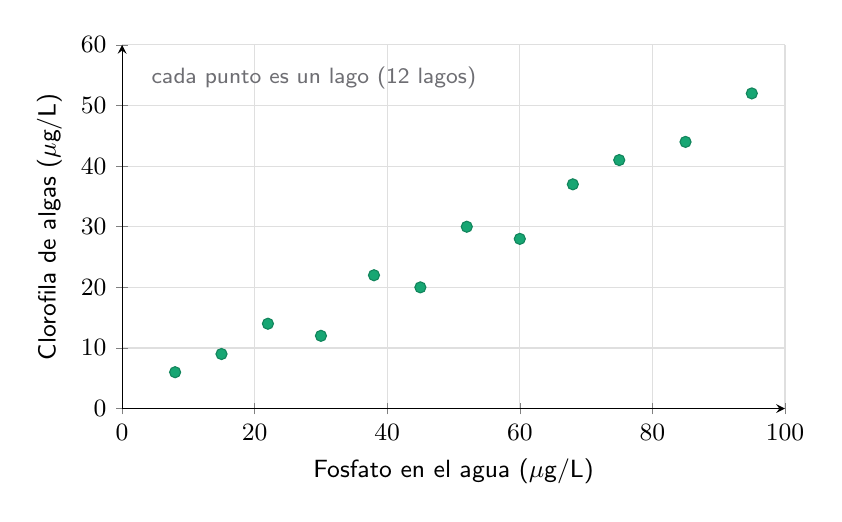
\begin{tikzpicture}[font=\small]
\begin{axis}[width=10cm,height=6.2cm,axis lines=left,xmin=0,xmax=100,ymin=0,ymax=60,xtick={0,20,...,100},ytick={0,10,...,60},
  grid=major,grid style={gray!25},xlabel={Fosfato en el agua ($\mu$g/L)},ylabel={Clorofila de algas ($\mu$g/L)},clip=false]
\addplot[only marks,mark=*,menta!80!black,mark options={fill=menta,scale=1.0}] coordinates {(8,6)(15,9)(22,14)(30,12)(38,22)(45,20)(52,30)(60,28)(68,37)(75,41)(85,44)(95,52)};
\node[font=\footnotesize,text=gris,anchor=north west] at (axis cs:3,58) {cada punto es un lago (12 lagos)};
\end{axis}
\end{tikzpicture}
\end{document}
